\documentclass[letterpaper,twocolumn,amsmath,amssymb,pre]{revtex4-1}
\usepackage{graphicx}% Include figure files
%\usepackage{breqn}
\usepackage{color}

\newcommand{\todo}[1]{\textcolor{red}{[TODO: #1]}}

\newcommand\thetamax{\theta_{\text{max}}}

\begin{document}
\title{Fundamental measure theory for hard polyhedra.}

\author{David Roundy}
\affiliation{Department of Physics, Oregon State University}
%\pacs{61.20.Ne, 61.20.Gy, 61.20.Ja}
%%%%%%%%%%%%%%%%%%%%%%%%%%%%%%%%%%%%%%%%%%%%%%%%%%%%%%%%%%%%
\begin{abstract}
  We develop a classical density functional for hard polyhedra.
\end{abstract}

\maketitle


%%%%%%%%%%%%%%%%%%%%%%%%%%%%%%%%%%%%%%%%%%%%%%%%%%%%%%%%%%%%
\section{Introduction}

Why study hard polyhedra? Hard spheres are the standard reference
system for essentially all fluids, but always have 12-fold
coordination.  A few very interesting liquids have tetrahedral
coordination, which is particularly significant when we consider the
freezing transition.  By studying hard polyhedra, we potentially can
develop a reference functional that can incorporate orientational
effects.  (For reference, an excellent review of hard-particle systems
is the following book chapter~\cite{tarazona2008chapter}.)

There have been several studies of non-spherical hard shapes.  At
least one omitted the rotational degrees of
freedom~\cite{cuesta1996cubes, cuesta1997dimensional,
  cuesta1997fundamental, buhot1998numerical, martinez1999fundamental,
  capitan2007hexagons,
  capitan2008phase, martinez2008fundamental}.  At least one included
the rotational degrees of freedom, treating each orientation as a
distinct species, resulting in a density that exists in more
dimensions than three, which was applied to systems with a high aspect
ratio, which undergo a nematic transition~\cite{schmidt2001density,
  esztermann2006density, harnau2008structure, hansen2009fundamental,
  hansen2010tensorial}.  It seems a good thing to have a density
functional that is more efficient, with fewer degrees of freedom to
optimize.  In particular, we are optimistic that one can do better for
``almost spherical'' polyhedra.

There has been simulation of the melting of hard cubes, demonstrating
that allowing rotational disorder leads to a first-order phase
transition~\cite{jagla1998melting}, which is not seen in parallel hard
cubes.  There has been another study of melting of parallel hard
cubes~\ref{groh2001closer}.

\section{Main ideas}

\newcommand\rr{\mathbf{r}}
\newcommand\rhat{\mathbf{\hat{r}}}
\newcommand\rot{\mathbf{\varpi}}

We will begin with the extension of fundamental measure theory (FMT)
to non-spherical particles by (so and so: add citation).  This theory
is based around a density that is a function of both position $\rr$
and orientation $\rot$.  The weighted densities are defined for a
given orientation, and then rotated appropriately when computing the
fundamental measures:
\begin{align}
  n_\alpha(\rr) &= \int n(\rr',\rot) w_\alpha(R(\rot)(\rr-\rr')) d\rr' d\rot
\end{align}
where $R(\rot)$ is the rotation operator corresponding to the
orientation $\rot$, and $w_\alpha(\rr)$ is the fundamental measure of
a single particle in the reference orientation at the origin.

Given these fundamental measures, the free energy is computed with
the standard Rosenfeld formula, plus a single correction, which we
will discuss later.
\begin{align}
  A_{HS} &= k_BT \int \Phi(\{n_\alpha(\rr)\}) d\rr
\end{align}

We propose to treat the orientational dependence of the fundamental
measures using an expansion in spherical harmonics:
\begin{align}
  w_\alpha(\rr) &= \sum_{lm} \tilde{w}_\alpha^{lm}(|\rr|) Y_{lm}(\rhat)
\end{align}
Given this expansion, we can simplify the weighted densities:
\begin{align}
  n_\alpha(\rr) &= \int \sum_{lm} n(\rr',\rot)
  \tilde{w}_\alpha^{lm}(|\rr-\rr'|)
  Y_{lm}(\widehat{R(\rot)(\rr-\rr')}) d\rr' d\rot
  \\
  &= \sum_{lmm'} \int \tilde{w}_\alpha^{lm}(|\rr-\rr'|)
  Y_{lm'}(\widehat{(\rr-\rr')})
  n(\rr',\rot)
       D_{lmm'}(\rot) d\rot d\rr'
       \\
  &=
    \sum_{lmm'} \int \tilde{w}_\alpha^{lm}(|\rr-\rr'|)
    Y_{lm'}(\widehat{(\rr-\rr')})
    n_{lmm'}(\rr') d\rr'
\end{align}
This reduces the challenge of handling the rotation to that of solving
for a set of densities $n_{lmm'}(\rr)$.

\subsection{Ideal gas free energy}
To address this, we will
first consider the free energy of an ideal gas.
\begin{widetext}
\begin{align}
  A_{\textit{ideal}} &=
  k_BT \int
  \left(n(\rr,\rot)\ln(\Lambda^3\Theta^3 n(\rr,\rot)) - n(\rr,\rot)
  \right) d\rr d\rot \label{eq:Aideal}
  \\
  &=
  k_BT \sum_{lmk} \int
  n_{lmk}(\rr)D_{lmk}(\rot)\left(
  \ln\left(\Lambda^3\Theta^3 \sum_{l'm'k'} n_{l'm'k'}(\rr)D_{l'm'k'}(\rot)\right) - 1
  \right) d\rr d\rot
  \\
  &=
  k_BT 8\pi^2 n_{000}(\rr)( \ln(\Lambda^3\Theta^3) - 1) +
  k_BT \sum_{lmk} \int
  n_{lmk}(\rr)D_{lmk}(\rot)
  \ln\left(n_{000}(\rr) + \sum_{\substack{l'>0\\m'k'}} n_{l'm'k'}(\rr)D_{l'm'k'}(\rot)\right)
  d\rr d\rot
  \\
  &=
  k_BT 8\pi^2 n_{000}(\rr)( \ln(\Lambda^3\Theta^3n_{000}(\rr)) - 1) +
  k_BT \sum_{lmk} \int
  n_{lmk}(\rr)D_{lmk}(\rot)
  \ln\left(1 + \sum_{\substack{l'>0\\m'k'}} \frac{n_{l'm'k'}}{n_{000}(\rr)}(\rr)D_{l'm'k'}(\rot)\right)
  d\rr d\rot
  \\
  &=
  k_BT 8\pi^2 n_{000}(\rr)( \ln(\Lambda^3\Theta^3n_{000}(\rr)) - 1)
  \\&\quad+
  k_BT \sum_{lmk} \int
  n_{lmk}(\rr)D_{lmk}(\rot)
  \left(\sum_{\substack{l'>0\\m'k'}}
  \frac{n_{l'm'k'}(\rr)}{n_{000}(\rr)}D_{l'm'k'}(\rot)
  - \frac12 \left(\sum_{\substack{l'>0\\m'k'}}
    \frac{n_{l'm'k'}(\rr)}{n_{000}(\rr)}D_{l'm'k'}(\rot)
  \right)^2
  + \cdots \right)
  d\rr d\rot
  \\
  &=
  k_BT 8\pi^2 n_{000}(\rr)( \ln(\Lambda^3\Theta^3n_{000}(\rr)) - 1)
  %\\&\quad
  +
  k_BT \sum_{l>0mk}
  \frac{8\pi^2}{2l+1}\frac{|n_{l'm'k'}(\rr)|^2}{n_{000}(\rr)}
  - \frac12 \frac{8\pi^2}{2l+1}\frac{|n_{l'm'k'}(\rr)|^2}{n_{000}(\rr)}
  + \cdots \label{eq:integrated}
  \\
  &=
  k_BT 8\pi^2 n_{000}(\rr)( \ln(\Lambda^3\Theta^3n_{000}(\rr)) - 1)
  +
  k_BT \sum_{l>0mk}
  \frac{4\pi^2}{2l+1}\frac{|n_{l'm'k'}(\rr)|^2}{n_{000}(\rr)}
  + \cdots \\
  &\approx
  k_BT 8\pi^2 n_{000}(\rr)( \ln(\Lambda^3\Theta^3n_{000}(\rr)) - 1)
  -
  \frac{n_{000}(\rr)}{2}k_BT \ln\left(1 - \sum_{l>0mk}
  \frac{8\pi^2}{2l+1}\frac{|n_{l'm'k'}(\rr)|^2}{n_{000}(\rr)}
  \right) \label{eq:approxideal}
\end{align}
\end{widetext}
In Equation~\ref{eq:integrated} we have used the fact that
$D_{000}(\rot)=1$, and because $n(\rr,\rot)$ is real, $n_{l,-m,-k} =
n_{lmk}^*$.  In Equation~\ref{eq:approxideal}, we have constructed an
approxmation to the ideal gas free energy which has the correct
first-order response in the orientational order $n_{l>0,mk}(\rr)$ and
diverges (as it should) when $n_{l>0,mk}(\rr) \gg n_{000}(\rr)$, which
would lead to the nonsense result that $n(\rr,\rot) < 0$.  We can tune
the divergence a bit by moving constant factors (e.g. $8\pi^2$ into
our out of the logarithm.

\subsection{Finding the orientational moments}
We find the orientational moments $n_{lmm'}(\rr)$ by minimizing the
free energy.  Let's begin by optimizing the free energy with respect
to nonzero angular momenta:
\begin{align}
  0&=\frac{\delta A}{\delta n_{lmm'}(\rr)} \\
  &= \frac{2l+1}{8\pi^2}n_{lmm'}(\rr)
  + k_BT \int\sum_\alpha
  \frac{\partial \Phi(\rr')}{\partial n_\alpha(\rr')}
  \frac{\delta n_\alpha(\rr')}{\delta n_{lmm'}(\rr)} d\rr'
  \\
  &=
   \frac{2l+1}{8\pi^2}n_{lmm'}(\rr)
  \\&\quad+ k_BT \int\sum_\alpha
  \frac{\partial \Phi(\rr')}{\partial n_\alpha(\rr')}
  \tilde{w}_\alpha^{lm}(|\rr-\rr'|)Y_{lm'}(\widehat{\rr-\rr'}) d\rr'
\end{align}
Solving for $n_{lmm'}(\rr)$, we find that
\begin{align}\label{eq:nlmm'}
  n_{lmm'}(\rr) &= \frac{8\pi^2k_BT}{2l+1}
  \int\sum_\alpha
  \frac{\partial \Phi(\rr')}{\partial n_\alpha(\rr')}
  \tilde{w}_\alpha^{lm}(|\rr-\rr'|)Y_{lm'}(\widehat{\rr-\rr'}) d\rr'
\end{align}
I note that this equation for $n_{lmm'}$ is approximate, since we made
an approximation when we neglected higher order terms in the expansion
of the log in the ideal gas free energy.  Thus in cases where there is
relatively little orientational ordering, it ought to be an accurate
equation.

In cases where $n_{lmm'} \approx n_{000}$, we could reasonbly become
concerned that $n(\rr, \rot)$ could become negative for some
orientations, which would be unphysical.  If this becomes a problem,
we would want to address it by including nonlinear effects of the
$\ln$ in Equation~\ref{eq:Aideal}.  For now, let's stick with the
linear approximation, and hope for the best.  If we find that
$n_{lmm'} > n_{000}$ in practice, we would want to revisit this
decision, and make use of something like
Equation~\ref{eq:approxideal}.


\subsection{The Procedure}
Our input when computing the free energy is the ordinary density
$n(\rr)$, which is precisely equal to $n_{000}(\rr)$ above, because it
is just the orientationally averaged density, which is also what
$n_{000}(\rr)$ is.  From this density, we can compute a first set of
fundamental measures
\begin{align}
  n_\alpha(\rr) &= \int \tilde{w}_\alpha^{000}(|\rr-\rr'|)n(\rr')d\rr'
\end{align}
where we will discuss elsewhere how we find the weighting functions
$\tilde{w}_\alpha^{000}$.  Thus we have our zeroth-order approximation
to the fundamental measures.  At this point we can compute a
zeroth-order free energy just by evaluating the free energy functional
with these fundamental measures, which would be the true free energy
if there were no orientational ordering.

From the zeroth-order fundamental measures, we can
compute the orientational densities using Eq.~\ref{eq:nlmm'}.  Once we
have these densities, we can find an improved set of fundamental
measures:
\begin{align}
  n_\alpha(\rr) &= \sum_{lmm'} \int
  \tilde{w}_\alpha^{lm}(|\rr-\rr'|) Y_{lm'}(\rr-\rr')n_{lmm'}(\rr')
\end{align}
With this improved set of fundamental measures, we can now just
evaluate the free energy.  How could it be simpler? Well, it could be
more complicated if we were to go back and try to compute an improved
set of $n_{lmm'}(\rr)$ using our improved fundamental measures.  I
suspect this would be silly, since we have already dropped out cubic
terms in $A_{\textit{ideal}}$.  No benefit from precisely computing a
higher order correction to a low-order approximation.  It \emph{is}
worth checking (particularly while debugging) that our two
approximations for the fundamental measures aren't \emph{too} wildly
different, and that the two approximations to the free energy also
aren't too wildly different.

\subsection{Finding the $000$ weighting functions for any polyhedron}

\newcommand\xhat{\mathbf{\hat{x}}}
\newcommand\yhat{\mathbf{\hat{y}}}
\newcommand\zhat{\mathbf{\hat{z}}}
\newcommand\facehat{\mathbf{\hat{f}}}
\newcommand\Rface{\ensuremath{R_f}}
\newcommand\Rvertex{\ensuremath{R_v}}

Here I will discuss how to find the weighted densities we need in
order to study polyhedra.  I will attempt in this section to evaluate
the $000$ weighting function for an arbitrary polyhedron, specified in
terms of the locations of its vertices and face centers (and possibly
also edge centers, although they should be computable from the vertex
and face radii).

\subsubsection{$w_3$}
We begin with the packing fraction $n_3(\rr)$.
\begin{align}
  w_3(\rr) &= 1 \text{ inside the polyhedron}\\
  &= 0 \text{ outside the polyhedron} \\
  &= \prod_i^{\text{faces}} \Theta(\Rface - \rr\cdot\facehat_i)
\end{align}
This is pretty easy, although the integrals will be less so.  The
$000$ integral is always going to give us something that is
essentially the same.  This integral is simply:
\begin{align}
  w_3^{000}(r) = \int w_3(\rr') \delta(|\rr'|-r) d^3r'\label{eq:w3000}
\end{align}
or we could write it as an integral over solid angle:
\begin{align}
  w_3^{000}(r) = \int w_3(\rr) d\Omega
\end{align}
Let's suppose we have $N$ faces and $M$ vertices per face.  If the
face center is at radius $\Rface$ and the vertex is at radius $\Rvertex$, then
we can compute $w_3^{000}$ by integrating over the irregular
tetrahedron enclosed by the for radii given by one vertex, one edge
center and one face center, as depicted in Figure~\ref{fig:r3000}, and
multiplying by $NM$ to account for the entire volume.  By doing this,
we can solve once for $w_3^{000}(r)$ for any regular polyhedron.

\begin{figure}
\includegraphics[width=\columnwidth]{figs/w3-000}
\caption{How we integrate for arbitrary polyhedron.}\label{fig:r3000}
\end{figure}

To begin, we solve for the positions of the vertices, which are shown
in Figure~\ref{fig:r3000}.  To perform our integration, as in
Equation~\ref{eq:w3000}, we will choose a coordinate system in which
the center of the face is in the $\xhat$ direction, and the line from the
center of the face to the center of the edge is in the $\yhat$
direction.  Our integral then becomes:
\begin{widetext}
\begin{align}
  w_3^{000}(r) &= \int w_3(\rr') \delta(|\rr'|-r) d^3r'
  \\
  &= NM \int_0^{\Rface} dx
  \int_0^{\sqrt{\Rvertex^2-\Rface^2}\cos\left(\frac{2\pi}{M}\right)} dy
  \int_0^{y\tan\left(\frac{2\pi}{M}\right)} dz \delta(r - \sqrt{x^2 +
    y^2 + z^2})
\end{align}
\end{widetext}
This integral gives a piecewise smooth result, with different forms
when $r<\Rface$, $\Rface<r<R_e$, $R_e<r<\Rvertex$ and $\Rvertex<r$ (when it is zero).

\todo{Do the above integral}

\subsubsection{$w_2$}
$n_2(\rr)$ is the area, which we can easily get from the above
weighted density.
\begin{align}
  w_2(\rr) &= |\nabla w_3(\rr)| \\
  &= \sum_i^{\text{faces}} \delta(\Rface-\rr\cdot\facehat_i)
  \prod_{j\ne i} \Theta(\Rface-\rr\cdot\facehat_j)
\end{align}
Using the same notation as in the previous section, the integral
for $w_2^{000}$ becomes:
\begin{widetext}
\begin{align}
  w_2^{000}(r) &= \int w_2(\rr') \delta(|\rr'|-r) d^3r'
  \\
  &= NM
  \int_0^{\sqrt{\Rvertex^2-\Rface^2}\cos\left(\frac{2\pi}{M}\right)} dy
  \int_0^{y\tan\left(\frac{2\pi}{M}\right)} dz \delta(r - \sqrt{\Rface^2 +
    y^2 + z^2})
\end{align}
\end{widetext}
This integral gives a piecewise smooth result, with different forms
when $r<\Rface$ (it is zero), $\Rface<r<R_e$, $R_e<r<\Rvertex$ and $\Rvertex<r$ (it is
zero).

\todo{Do the above integral}

\subsubsection{$w_1$}

$n_1(\rr)$ is the first fundamental measure that is interestingly
different for polyhedra than it is for spheres.  This is a measure of
the mean curvature, and polyhedra have no curvature except at the
edges.  Thus $n_1(\rr)$ is going to be nonzero only on the edges, and
there it will be a delta function.
\begin{align}\label{eq:w1}
  w_1(\rr) &= \sum_{ij}^{\text{NN faces}}
  \Theta\left(\Rvertex - r\right)
  \delta(\Rface - \rr\cdot \facehat_i)
  \delta(\Rface - \rr\cdot \facehat_j)
\end{align}
where $\facehat_i$ is a unit vector in the direction of the $i$ face
of the polyhedron, $\Rvertex$ is the distance between the center of
the polyhedron and the vertex, and $\Rface$ is the distance of the
center of the face from the origin.  \todo{WARNING: I may have something off
in these formulas, but the general idea is there.  To check on a
constant factor that may be off, we could check that the result
approaches the spherical value for a dodecahedron.  If it's off, it's
likely off by a largish factor.}

As before, we should be able to do this integral for $w_1^{000}$
independently of the specific polyhedron in question.  Our choice of
coordinates will be different, as we only want to integrate over the
edge, so we may as well put the edge center on the $\xhat$ axis, and
the edge itself along the $\yhat$ axis.
\begin{align}
  w_1^{000}(r) &= \int w_1(\rr') \delta(|\rr'|-r) d^3r'
  \\
  &= NM \text{constant factor}
  \int_0^{\sqrt{\Rvertex^2-\Rface^2}\sin\left(\frac{2\pi}{M}\right)} dy
  \delta(r - \sqrt{R_e^2 + y^2})
\end{align}
The only tricky bit is to get this constant factor right, which will
relate to the angle between adjacent faces.

\todo{Do this integral}

\todo{Find the constant factor}

\subsubsection{$w_0$}

$n_0(\rr)$ is the fundamental measure of gaussian curvature, which is
the product of the curvature in the two eigendirections.  This is zero
(for polyhedra) except at the corners, so $n_0(\rr)$ itself is going
to be zero except at the corners.  Also, the gaussian curvature
must satisfy a sum rule, which tells us that
\begin{align}
  w_0(\rr) &= \frac1{N}\sum_{i}^{N\text{ vertices}} \delta(\rr-\rr_i)
\end{align}
Interestingly, this means that
\begin{align}
  w_0^{000}(\rr) &= \frac{\delta(\Rvertex - |\rr|)}{4\pi \Rvertex^2}
\end{align}
which means that as far as $w_0^{000}$ is concerned, the polyhedron is a
sphere with a radius equal to the vertex distance (i.e. the distance
from the center to the vertex of the polyhedron).

\subsubsection{$\mathbf{w_{2V}}$}

\todo{TODO}

\subsubsection{$\mathbf{w_{1V}}$}

\todo{TODO}

\subsection{Tetrahedron}

\subsubsection{$w_3^{000}$}

In order to solve for $w_3^{000}(r)$ of a tetrahedron, we need to
consider where $r$ lies.  If $r<\frac{\sqrt{3}}{2}R$ (which is
\Rface), then the sphere lies entirely within the tetrahedron, and
$w_3^{000}(r)=1$.  Conversely, if $r<\sqrt{3}R$ (which is \Rvertex),
then $w_3^{000}(r)=0$.  There are two in-between cases:  either
$R<r<\Rvertex$ (in which case each vertex forms an isolated triangle
poking out of the sphere), or $\Rface<r<R$, in which case isolated
circles of spherical surface poke out of the faces of the
tetrahedron.  The latter case is pretty easy, if we just integrate
over the sticking-out bits, and subtract that from the total surface
area of the sphere:
\begin{align}
  w_3^{000}(r) &= 1 - \frac1{\pi}\int d\Omega \\
  &= 1 - \frac1{\pi}2\pi \int_0^{\cos^{-1}\left(\frac{\sqrt{3}R}{2r}\right)} \sin\theta d\theta
  \\
  &= 1 - 2 \int^1_{\frac{\sqrt{3}R}{2r}} du
  \\
  &= \frac{\sqrt{3}R}{r} - 1
  \\
  \frac{\sqrt{3}R}{2}&<r<R
\end{align}

The final consideration (for $w_3^{000}(r)$ of a tetrahedron) is when
$R < r < \sqrt{3}R$, when we will want to just integrate over the
curvy triangles formed by the portion of the tetrahedron that stick
through the sphere.  We just need to integrate through one of these
points, and multiply by four... which might be easiest to do in a
Cartesian coordinates rotated by 45$^\circ$ around the ordinary $z$
axis.
\begin{widetext}
\begin{align}
  w_3^{000}(r)
  &=
  \frac4{4\pi r^2}
  \int_{0}^R dz
  \int_0^{\frac{R+z}{\sqrt{2}}} dy
  \int_0^{\frac{R-z}{\sqrt{2}}} dx
  \delta(r-\sqrt{x^2+y^2+z^2})
  \\
  &=
  \frac1{\pi r^2}
  \int_{0}^R dz
  \int_0^{\frac{R+z}{\sqrt{2}}} dy
  \int_{\frac{z-R}{\sqrt{2}}}^{\frac{R-z}{\sqrt{2}}} dx
  \delta(r-\sqrt{x^2+y^2+z^2})
  \\
  u&= \sqrt{x^2+y^2+z^2}\\
  du &= \frac{ydy}{\sqrt{x^2+y^2+z^2}}
  \\
  w_3^{000}(r)
  &=
  \frac1{\pi r^2}
  \int_{0}^R dz
  \int_{\frac{z-R}{\sqrt{2}}}^{\frac{R-z}{\sqrt{2}}} dx
  \int_{\sqrt{z^2+x^2}}^{\sqrt{x^2+z^2+\frac{(R+z)^2}{2}}} du
  \delta(r-u)\frac{u}{\sqrt{u^2-z^2-x^2}}
  \\
  &=
  \frac1{\pi r^2}
  \int_{\sqrt{r^2-2R^2}}^R dz
  \int_{\frac{z-R}{\sqrt{2}}}^{\frac{R-z}{\sqrt{2}}} dx
  \int_{\sqrt{z^2+x^2}}^{\sqrt{x^2+z^2+\frac{(R+z)^2}{2}}} du
  \delta(r-u)\frac{u}{\sqrt{u^2-z^2-x^2}}
  \\
  z^2+x^2+y^2 &= r^2 \\
  z_{min}^2 + (R-z_{min})^2/2 &= r^2
\end{align}
Instead I'm going now to think of using cylindrical coordinates...
\begin{align}
  w_3^{000}(r) &= 3\frac{4}{4\pi r^2}
  \int_0^{\sqrt{3}R}dz\int_{-\frac{\pi}{3}}^{\frac{\pi}{3}}d\phi\int_0^{2\frac{\sqrt{3}R-z}{\cos\phi}} ds
  \delta(r-\sqrt{z^2+s^2})
  \\
  &= \frac{3}{\pi r^2}
  \int_0^{\sqrt{3}R}dz\int_{-\frac{\pi}{3}}^{\frac{\pi}{3}}d\phi\int_0^{2\frac{\sqrt{3}R-z}{\cos\phi}} ds
  \delta(r-\sqrt{z^2+s^2})
  \\
  u &= z^2+s^2 \\
  du &= sds \\
  &= \frac{\sqrt{u^2-z^2}}{u}ds
  \\
  w_3^{000}(r)
  &= \frac{3}{\pi r^2}
  \int_0^{\sqrt{3}R}dz\int_{-\frac{\pi}{3}}^{\frac{\pi}{3}}d\phi\int_{z}^{\sqrt{z^2+\left(2\frac{\sqrt{3}R-z}{\cos\phi}\right)^2}} du
  \delta(r-u)\frac{u}{\sqrt{u^2-z^2}}
  \\
  R &= \frac{2}{\sqrt{3}}s\cos\phi + \frac{1}{\sqrt{3}}z \\
  s &= 2\frac{\sqrt{3}R-z}{\cos\phi}
\end{align}
Maybe spherical coordinates? Rotated $\pi/4$? Let's look first at the
plane that is our limit for $\theta$:
\begin{align}
  \sqrt{3}R &= x + y + z \\
  &= \sqrt{2}r\sin\thetamax\cos\phi +
  r\cos\thetamax
  \\
  \sqrt{3}\frac{R}{r} &=
  \sqrt{2}\sqrt{1-\cos^2\thetamax}\cos\phi
  + \cos\thetamax
  \\
  \sqrt{1-\cos^2\thetamax} &=
  \frac{\sqrt{3}\frac{R}{r}-\cos\thetamax}{\sqrt{2}\cos\phi}
  \\
  1-\cos^2\thetamax &=
  \frac{3\frac{R^2}{r^2}+\cos^2\thetamax -
    2\sqrt{3}\frac{R}{r}\cos\thetamax}{2\cos^2\phi}
  \\
  0 &=
  (1+2\cos^2\phi)\cos^2\thetamax
  - 2\sqrt{3}\frac{R}{r}\cos\thetamax
  + \left(3\frac{R^2}{r^2} - 2\cos^2\phi\right)
  \\
  \cos\thetamax &= \frac{2\sqrt{3}\frac{R}{r}
  - \sqrt{12\frac{R^2}{r^2} - 4(1+2\cos^2\phi)\left(3\frac{R^2}{r^2}-2\cos^2\phi\right)}}{2(1+2\cos^2\phi)}
  \\
  &= \frac{\sqrt{3}\frac{R}{r}
  - \sqrt{3\frac{R^2}{r^2} -
    (1+2\cos^2\phi)\left(3\frac{R^2}{r^2}-2\cos^2\phi\right)}}{1+2\cos^2\phi}
  \\
  &= \frac{\sqrt{3}\frac{R}{r}
  - \sqrt{3\frac{R^2}{r^2} - (2-\cos2\phi)\left(3\frac{R^2}{r^2}-1+\cos2\phi\right)}}{2-\cos2\phi}
\end{align}
\end{widetext}
This is sort of a mess, but does look useable.
\begin{align}
  w_3^{000}(r) &=
  \frac{12}{4\pi}
  \int_{-\frac{\pi}{3}}^{\frac{\pi}{3}}d\phi
  \int_0^{\thetamax}d\theta
  \sin\theta
  \\
  &=
  \frac{3}{\pi}
  \int_{-\frac{\pi}{3}}^{\frac{\pi}{3}}
  (1 - \cos\thetamax)d\phi
\end{align}
Surely we can either use Euler's relation or a geometrical
construction to solve for $\thetamax$?!

\subsubsection{$w_2^{000}$}
The easiest way to get $w_2^{000}(r)$ is just to take a derivative of
$w_3^{000}(r)$ we should have just computed:
\begin{align}
  w_2^{000}(r) &= \frac{dw_3^{000}(r)}{dr}
\end{align}

\subsubsection{$w_1^{000}$}
As mentioned before, $w_1^{000}(r)$ is the average of an integral
around the edges of the tetrahedron.  This is a little bit tricky, as
seen in Eq.~\ref{eq:w1}.  $w_1^{000}$ is zero except when $\sqrt{2}R <
r < \sqrt{3}R$.
\begin{align}
  \rr &= r\left(
  \sin\theta\cos\phi\xhat +
  \sin\theta\sin\phi\yhat +
  \cos\theta\zhat \right)
  \\
  \facehat_1 &= \frac{\xhat+\yhat+\zhat}{\sqrt{3}} \\
  \facehat_2 &= \frac{-\xhat-\yhat+\zhat}{\sqrt{3}} \\
  \rr\cdot\facehat_1 &=
  \frac{r}{\sqrt{3}}\left(
  \cos\theta+\sin\theta\cos\phi + \sin\theta\sin\phi
  \right)
  \\
  &= \frac{r}{\sqrt{3}}\left(
  \cos\theta+\sqrt{2}\sin\theta\cos(\phi+\pi/4)
  \right)
  \\
  \rr\cdot\facehat_2 &=
  \frac{r}{\sqrt{3}}\left(
  \cos\theta-\sqrt{2}\sin\theta\cos(\phi+\pi/4)
  \right)
\end{align}
\begin{widetext}
\begin{align}
  w_1^{000}(r) &= \frac{6}{4\pi}\int
  \delta(\sqrt{2}R - \rr\cdot \facehat_1)
  \delta(\sqrt{2}R - \rr\cdot \facehat_2)
  \sin\theta d\theta d\phi
  \\
  &= \frac{6}{4\pi}\int
  \delta\left(\sqrt{2}R
  - \frac{r}{\sqrt{3}}(\cos\theta-\sin\theta\cos(\phi+\pi/4))\right)
  \delta\left(\sqrt{2}R
  - \frac{r}{\sqrt{3}}(\cos\theta+\sin\theta\cos(\phi+\pi/4))\right)
  \sin\theta d\theta d\phi
\end{align}
\end{widetext}
\begin{align}
  u &= \sqrt{2}R -\frac{r}{\sqrt{3}}(\cos\theta + \sin\theta\cos(\phi+\pi/4)) \\
  du &= \frac{r}{\sqrt{3}}\sin\theta\sin(\phi+\pi/4)d\phi \\
  d\phi &= \frac{\sqrt{3}}{r\sin\theta}\frac{1}{\sin(\phi+\pi/4)}
  \\
  w_1^{000}(r)
  &= \frac{6}{4\pi}\int
  \delta\left(-2\frac{r}{\sqrt{3}}\cos\theta+u\right)
  \delta(u)
   \frac{\sqrt{3}}{r}\frac{ d\theta du}{\sqrt{1-u^2}OOPS!}
  \\
  &= \frac{6}{4\pi}\int
  \delta\left(-2\frac{r}{\sqrt{3}}\cos\theta\right)
   \frac{\sqrt{3}}{r}d\theta
   \\
  v &= -2\frac{r}{\sqrt{3}}\cos\theta \\
  dv &= 2\frac{r}{\sqrt{3}}\sin\theta d\theta \\
  &= 2\frac{r}{\sqrt{3}}\sqrt{1-v^2}d\theta \\
  w_1^{000}(r)
  &= \frac{6}{4\pi}\int
  \delta\left(v\right)
   \frac{6}{r^2}\frac{dv}{\sqrt{1-v^2}} \\
   &= \frac{9}{\pi r^2}
\end{align}
I'm a little doubtful of the above angular integral.  I don't see how
it will be able to integrate to anything very reasonable when
integrating over $r$.  In particular, I am pretty certain that
\emph{has} to depend on the distance of closest approach.
I know that
\begin{align}
  \int_{r_{min}}^{r} w_1^{000}(r)4\pi r^2dr
  &\propto \sqrt{r^2 - r_{min}^2}
\end{align}

\subsection{Cube}

In calculating $w_3^{000}$ we only need to integrate over one octant.
\begin{align}
  w_3^{000}(r) &= \int \Theta(R-x)\Theta(R-y)\Theta(R-z) d\Omega
  \\
  &= 8\int_0^{\frac{\pi}{2}} \int_0^{\frac{\pi}{4}}
  \Theta(R-r\sin\theta\cos\phi)
  \Theta(R-r\sin\theta\sin\phi)
  \Theta(R-r\cos\theta)
  r^2\sin\theta d\theta d\phi
  \\
  &=
  x
\end{align}
There are a couple of possibilities.  If $r<R$ then $w_3^{000}(r) =
1$.  If $r>\sqrt{3}R$ the $w_3^{000}(r) = 0$.  That leaves two
interesting possibilities.  If $R<r<\sqrt{2}R$ then there are six
edges to the integral, and we find that
\begin{align}
  w_3^{000}(r) &= \frac1{4\pi r^2}\int \Theta(R-x)\Theta(R-y)\Theta(R-z) d\Omega
\end{align}
If $\sqrt{2}R<r<\sqrt{3}R$ then there are just three sides to the
integral, as illustrated in Fig.~\ref{fig:rbig}.  This integral is
easiest to do by integrating over just one of the eight protruding
corners.  This seems easiest if we define the corner as the $z$ axis.
\begin{align}
  w_3^{000}(r) &= \frac{6}{4\pi}
  \int_{0}^{\frac{\pi}{3}}
  \int_0^{\theta_{m}} \sin\theta d\theta d\phi \\
  r\cos\theta_{m} + r\sin\theta_{m}\cos\phi  &= R
  \\
  \cos\theta_{m} + \sin\theta_{m}\cos\phi  &= \frac{R}{r} \\
  w_3^{000}(r) &= \frac{6}{4\pi}
  \int_{0}^{\frac{\pi}{3}}
  \int_0^{\theta_{m}} \sin\theta d\theta d\phi
\end{align}
\begin{align}
  w_3^{000}(r) &= \frac{8}{4\pi r^2}\iint_0^R \delta(r-\sqrt{x^2+y^2+z^2})
  dxdydz \\
  u &= \sqrt{x^2+y^2+z^2} \\
  du &= \frac{zdz}{u} \\
  w_3^{000}(r) &= \frac{8}{4\pi r^2}\iint_0^R \delta(r-u)
  dxdy\frac{udu}{\sqrt{u^2 -x^2-y^2}} \\
  &= \frac{2}{\pi r}\int_{r_0}^R\int_{r_0}^R
  dxdy\frac{1}{\sqrt{r^2 -x^2-y^2}} \\
  &= \frac{2}{\pi r}\int_{\sqrt{r^2-2R^2}}^R\int_{\sqrt{r^2-R^2-x^2}}^R
  \frac{dxdy}{\sqrt{r^2 -x^2-y^2}} \\
\end{align}
\begin{figure}
\includegraphics[width=2in]{figs/w3cube}
\caption{Picture of the sphere with $\sqrt{2}R<r<\sqrt{3}R$.}\label{fig:rbig}
\end{figure}

\bibliography{paper}% Produces the bibliography via BibTeX.

\end{document}
